\chapter{Condensadores}
\section{Generalidades}

Su funci\'on es condensar el fluido refrigerante proveniente del compresor (vapor sobrecalentado). El agente condensante puede ser aire o agua.El fluido entra en el condensador a la temperatura de descarga del compresor, \'este ir\'a intercambiando calor sensible con el entorno hasta llegar a la temperatura del condensaci\'on. Una vez llegado a esta temperatura se produce el cambio de estado a temperatura y presi\'on constante (calor latente). El calor total disipado en el condensador es la suma del calor que procede del evaporador m\'as el calor de trabajo del compresor. La temperatura de a la salida del condensador puede ser la de condensaci\'on o inferior (subenfriamiento). El subenfriamiento se puede producir en el mismo condensador y es positivo para el rendimiento de la instalaci\'on, o bien, se puede producir afuera de \'el en un intercambiador de calor.

\section{Capacidad de un condensador}

La capacidad de un condensador depende de la superficie del material, del tipo de material y de la diferencia de temperaturas entre los dos fluidos. Su valor es:
\begin{equation*}
    Q = S \cdot k \cdot \varDelta t
\end{equation*}
$Q = \text{cantidad de calor a disipar por el condensador}(kcal/h)$\\
$S = \text{superficie de transmisi\'on}(m^2)$\\
$k = \text{coeficiente de transmisi\'on del material}(kcal/(h \cdot m^2 \cdot \text{°C}))$\\
$\varDelta t = \text{diferencia de temperaturas entre el fluido refrigerante y el agente condensante(°C)}$

\section{Tipos de condensadores}

Se pueden clasificar seg\'un el agente condesante que se emplee sea agua o aire.

\subsection{Enfriados por agua}

\subsubsection{De doble tubo}

Tamb\'en conocidos como de contracorriente, consisten en dos tubos de distintos di\'ametros y conc\'entricos. El fluido refrigerante se descarga en el espacio anular comprendido entre los tubos conc\'entricos y circular en direcci\'on descendente hacia el recipiente acumulador. El agua circula en direcci\'on ascendente hacia el compresor, contraria al refrigerante.
\begin{figure}[h]
    \centering
    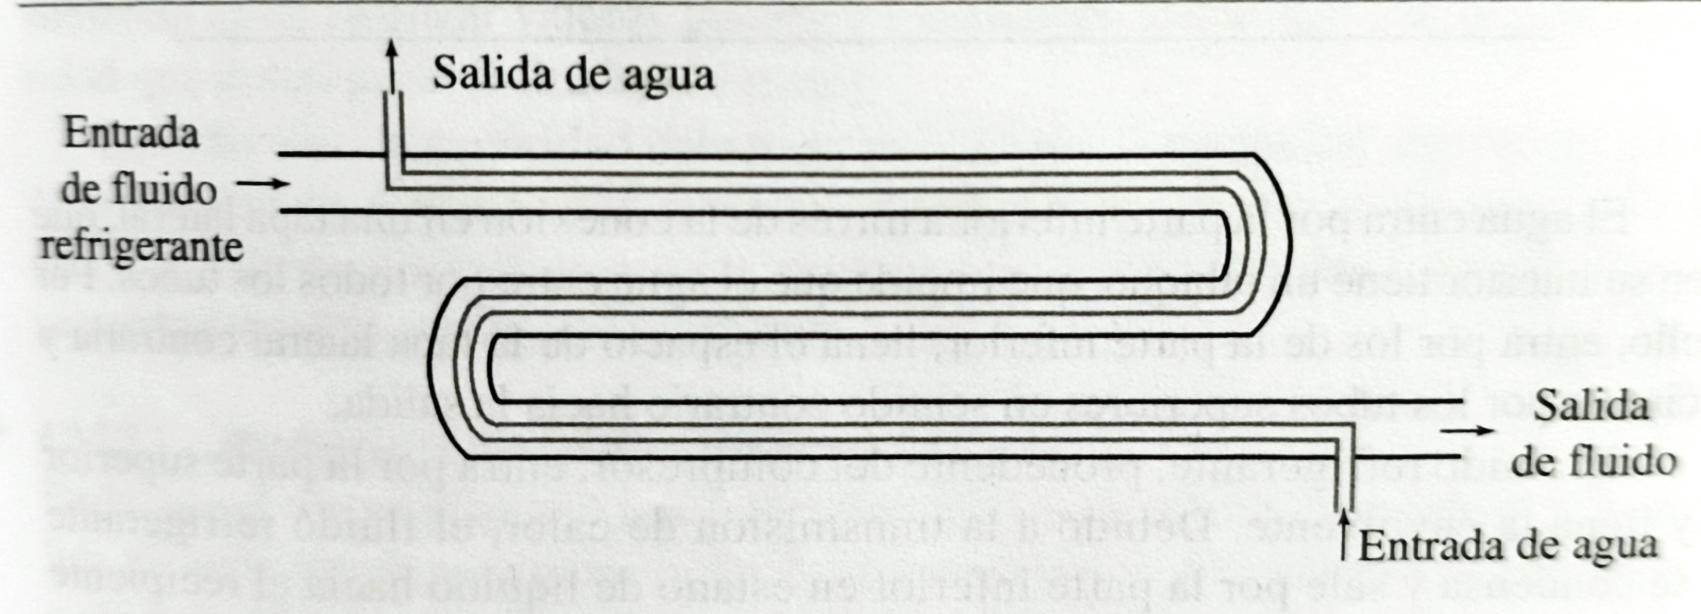
\includegraphics[width=.7\linewidth]{figuras/condensadores/condensador de doble tubo.jpg}
    \caption{Detalle de un condensador de doble tubo}
    \label{fig:Detalle de un condensador de doble tubo}
\end{figure}

\subsubsection{Multitubulares}

Est\'an formados por una envolvente met\'alica, de forma cil\'indrica, cerrada por los laterales por medio de unas tapas atornilladas que se pueden desmontar para inspecci\'on y mantenimiento. En el interior, a lo largo de la envolvente va montado el paquete tubular. Estos pueden ser verticales u horizontales.\\Los materiales que se utilizan en estos condensadores, var\'ian dependiendo del tipo de refrigerante empleado (por incompatibilidad) y el agente condensante, seg\'un sea agua dulce o agua de mar. Por ejemplo, la envolvente puede ser de acero y los tubos interiores de cobre cuando el agente condensante es agua de la red. O bien aleaci\'on cobre-n\'iquel o lat\'on aluminio, si es agua de mar. Con amon\'iaco, que es incompatible con el cobre, se emplea acero.
\begin{figure}[H]
    \centering
    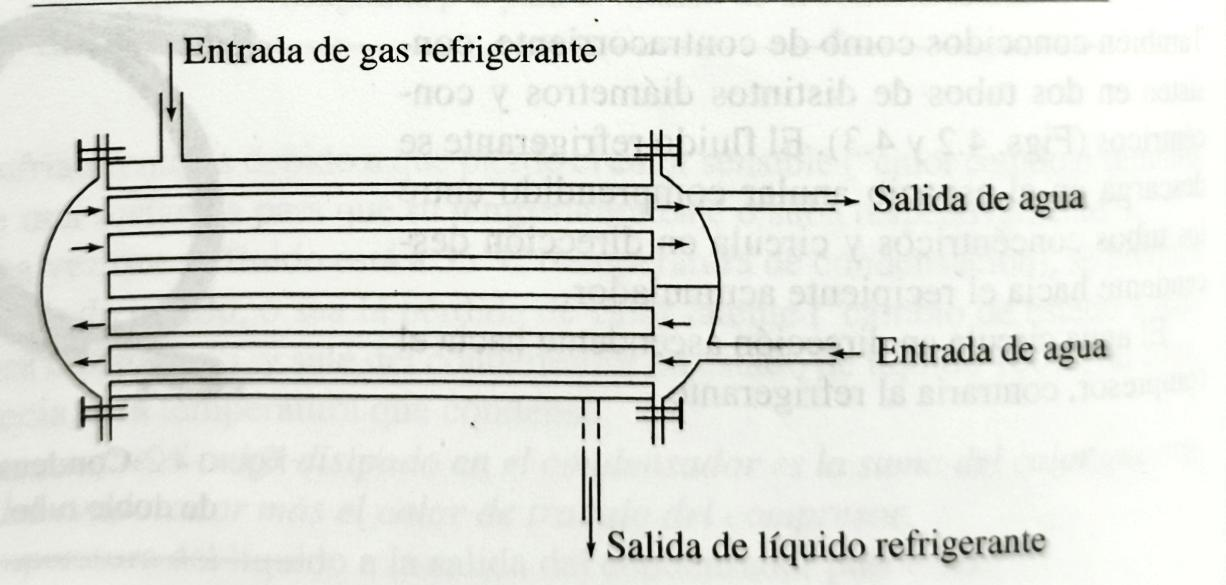
\includegraphics[width=0.6\linewidth]{figuras/condensadores/Condensador multitubular horizontal.jpg}
    \caption{Condensador multitubular horizontal}
    \label{fig:Condensador multitubular horizontal}
\end{figure}
El agua entra por la parte inferior a trav\'es de la conexi\'on en una tapa lateral, que en su interior tiene un tabique que impide que el agua entre por todos los tubos. Por ello, entra por los de la parte inferior, llena el espacio de la tapa lateral contraria y circula por los tubos superiores en sentido contrario hacia la salida.\\El fluido refrigerante, procedente del compresor, entra por la parte superior y llena la envolvente. Debido a la transmisi\'on de calor, el fluido refrigerante se condensa y sale por la parte inferior en estado l\'iquido hacia el recipiente acumulador.
\begin{figure}[H]
    \centering
    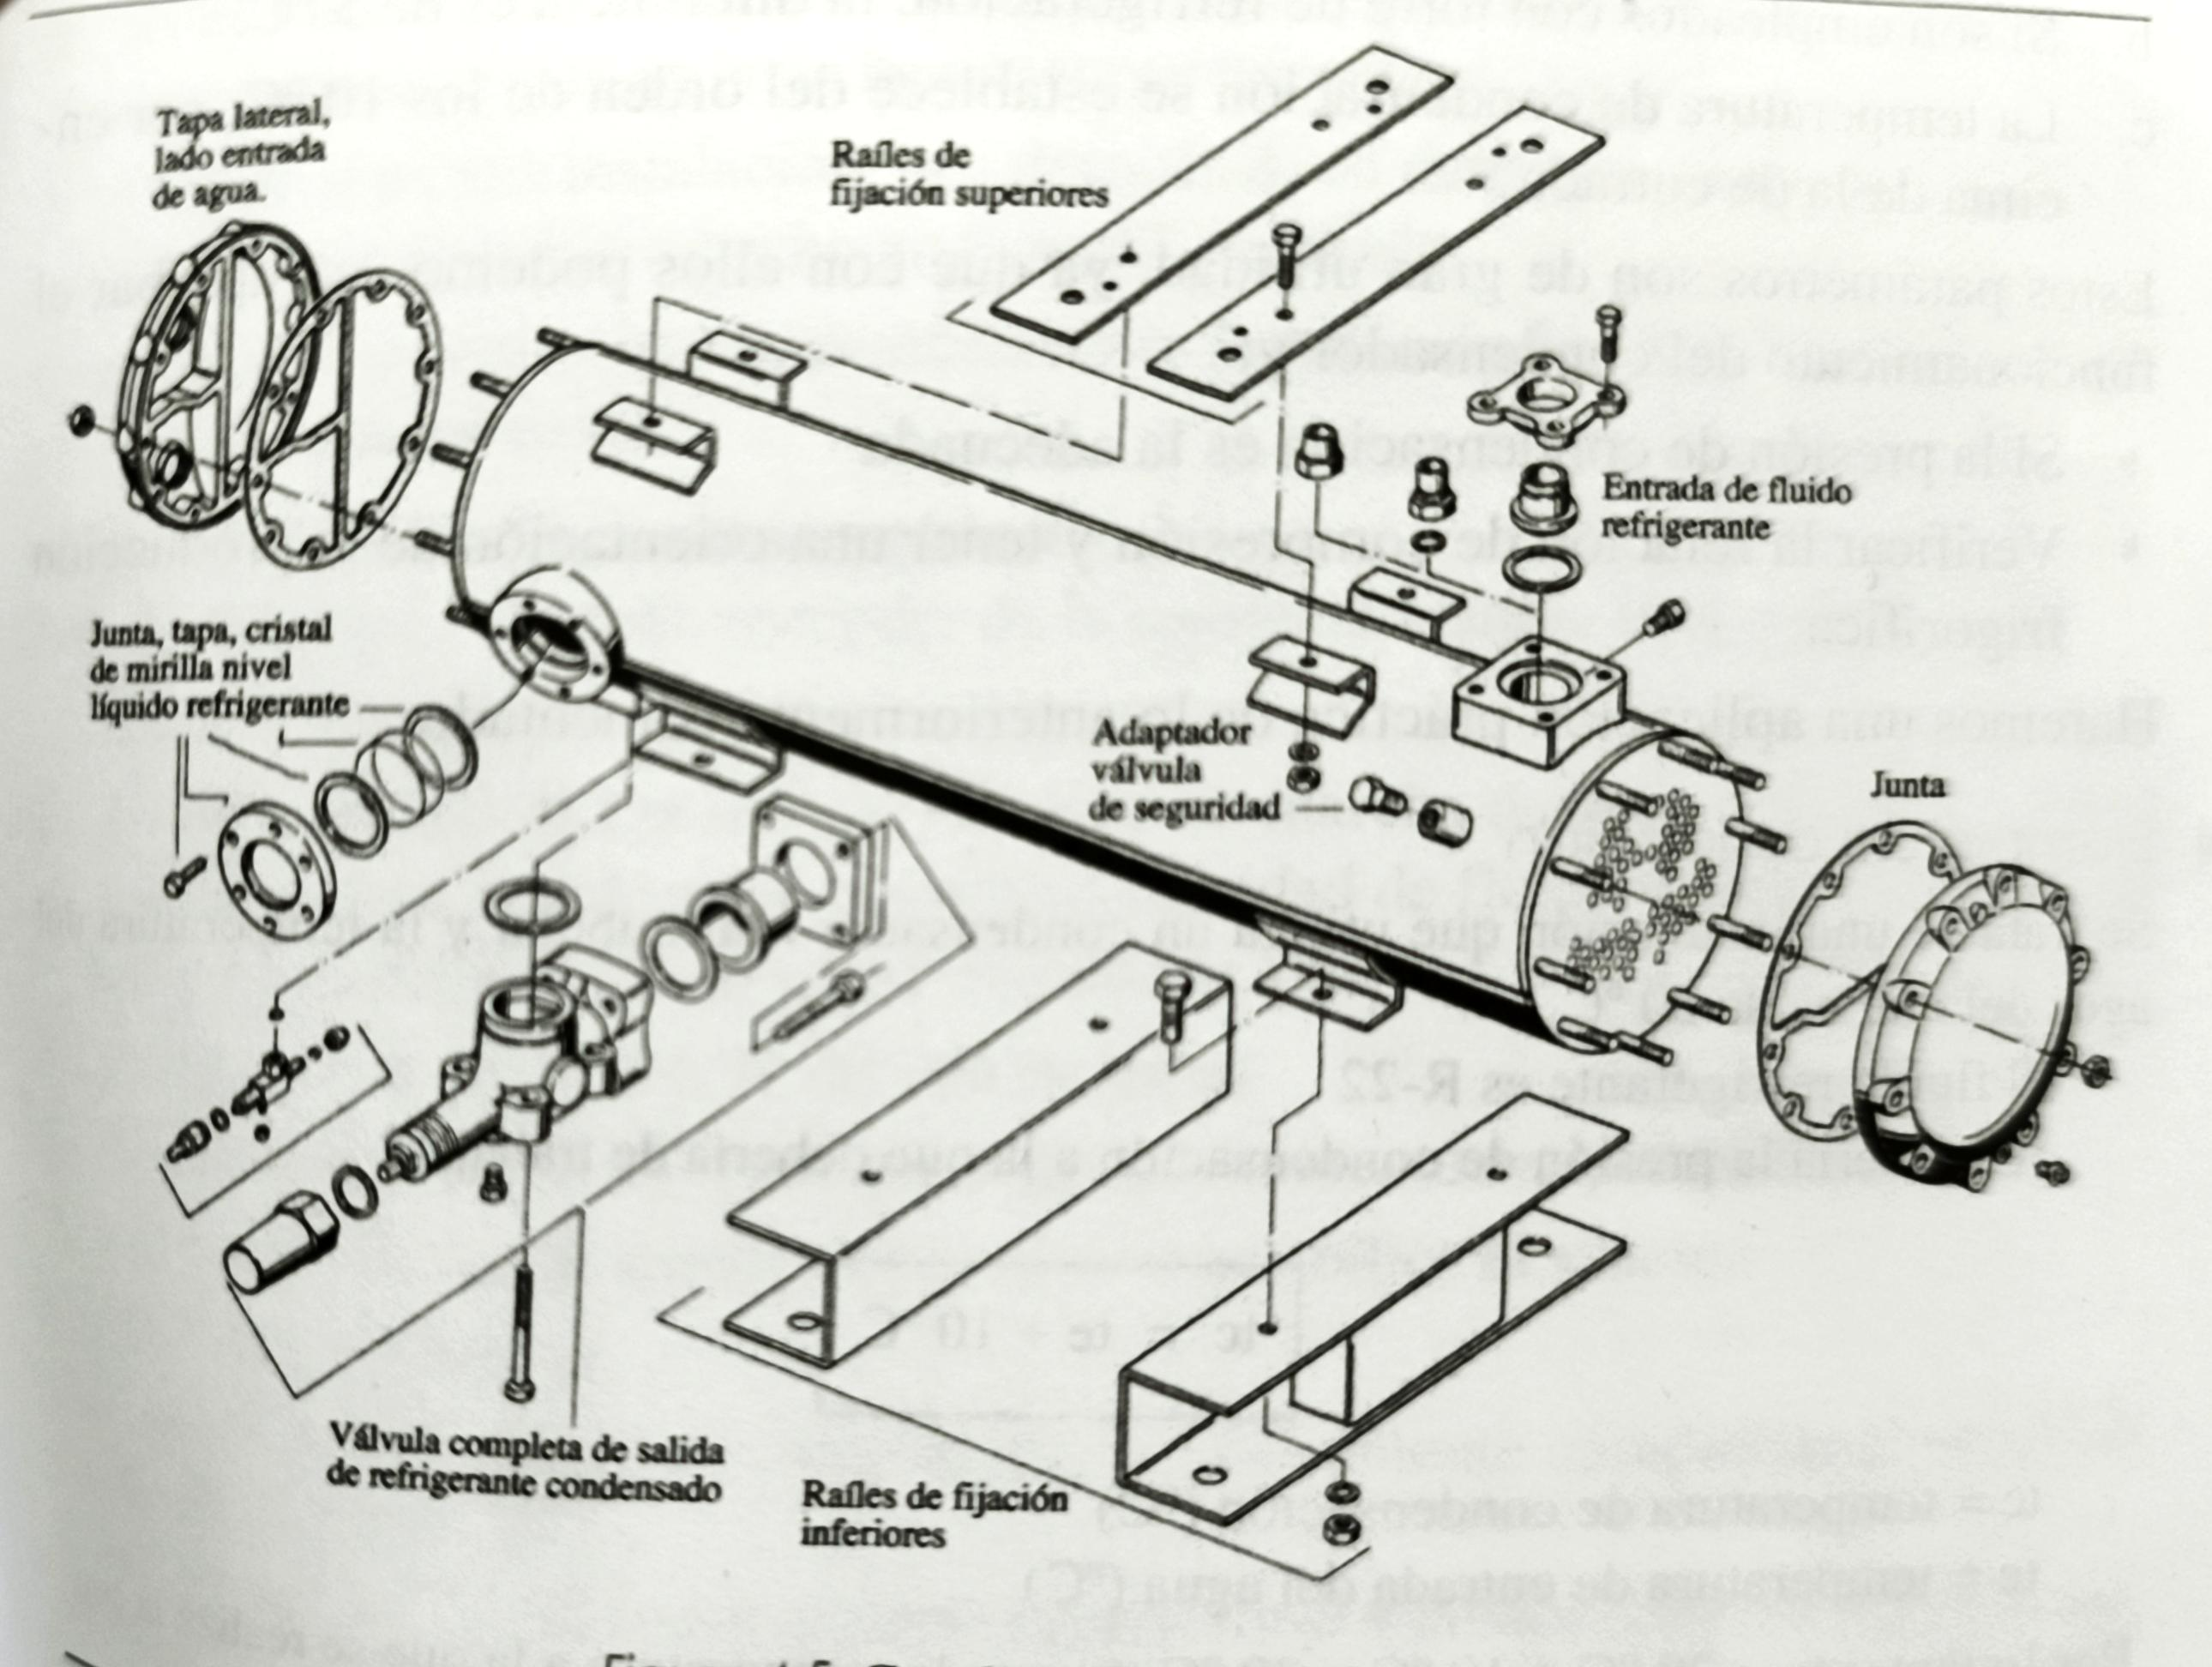
\includegraphics[width=0.6\linewidth]{figuras/condensadores/Despiece de condensador multitubular.jpg}
    \caption{Despiece de condensador multitubular}
    \label{fig:Despiece de condensador multitubular}
\end{figure}
Por lo general, los condensadores llevan instaladors en la parte superior de la envolvente dispositivos de seguridad y v\'alvula de purga para los gases incondensables.

\subsubsection{Par\'ametros de funcionamiento}

Dado que el agua se lleva el calor que disipa el condensador, \'esta sufrir\'a a la salida un aumento de temperatura. En los condensadores del tipo multitubulares, y a efectos pr\'acticos, se considera:
\begin{enumerate}[a.]
    \item Esa diferencia de temperaturas del orden de 5 \'o 6 \textcelsius.
    \item Si son empleados con torre de refrigeraci\'on, la diferencia es de 5 \textcelsius.
    \item La temperatura de condensaci\'on se establece del orden de los 10 \textcelsius, por encima de la entrada.
\end{enumerate}

Estos par\'ametros son de gran utilidad, ya que con ellos podemos comprobar el funcionamiento del condensador y:
\begin{itemize}
    \item Si la presi\'on de condensaci\'on es la adecuada
    \item Verificar la relaci\'on de compresi\'on y tener una orientaci\'on de la producci\'on frigor\'ifica
\end{itemize}
Tambi\'en a efectos de mantenimiento de la instalaci\'on, estos par\'ametros nos son de gran ayuda ya que, si por ejemplo, al cabo de un tiempo de funcionamiento:
\begin{enumerate}[a.]
    \item la presi\'on de condensaci\'on aumenta
    \item la presi\'on de baja se mantiene
    \item y la diferencia de temperaturas del agua disminuye, son s\'intomas de que el condensador est\'a sucio.
\end{enumerate}
O bien, si la presi\'on de condensaci\'on sube de manera anormal y la diferencia de temperaturas del agua aumenta, puede ser por falta de caudal (problemas en la bomba, filtro, v\'alvulas o taponamiento), pero si la diferencia no var\'ia, entonces es s\'intoma de gases incondensables en la instalaci\'on.

\subsubsection{Incondensables en el sistema}

Es uno de los problemas m\'as extendidos de la instalaci\'on, y puede ser debido a:
\begin{itemize}
    \item Que el compresor trabajando con una presi\'on de aspiraci\'on menor a la atmosf\'erica y aspire aire del ambiente
    \item Alteraci\'on qu\'imica del fluido refrigerante
    \item Alteraci\'on qu\'imica del aceite
    \item Luego de una operaci\'on de mantenimiento o puesta en marcha, que no se haya realizado correctamente el ``vac\'io''
\end{itemize}
\textbf{La presencia de gases incondensables en la instalci\'on implica el aumento de la presi\'on de condensaci\'on.}

\subsection{Enfriados por aire}

Los condensadores por aire pueden ser:

\subsubsection{De tubo liso}

Se emplean en instalaciones peque\~{n}as, como las heladeras dom\'esticas. El material es cobre y funcionan por circulaci\'on natural (convecci\'on natural). Es importante que tengan espacio libre para que el aire pueda circular, en caso contrario, podr\'ia elevarse la temperatura de condensaci\'on y con ello su presi\'on.

\subsubsection{De tubos con aletas}

Estos condensadores est\'an formados por un serpentin de cobre y aletas de aluminio separadas entre s\'i. La transmisi\'on de calor se produce a trav\'es del tubo y las aletas, con lo cual la superficie de transmisi\'on es mayor. Si, adem\'as, la circulaci\'on del aire es forzad mediante ventiladores, la capacidad del condensador aumenta. Este tipo de condensador es muy utilizado en instalaciones industriales.\\La \autoref{fig:Condensador_de_aire_forzado} representa un condensador de tubo con aletas de circulaci\'on forzada.\\La entrada de aire se realiza por la parte porterior del condensador, y la salida por la parte del lado de los ventiladores, siendo \'esta de menor secci\'on.
\begin{figure}[H]
    \centering
    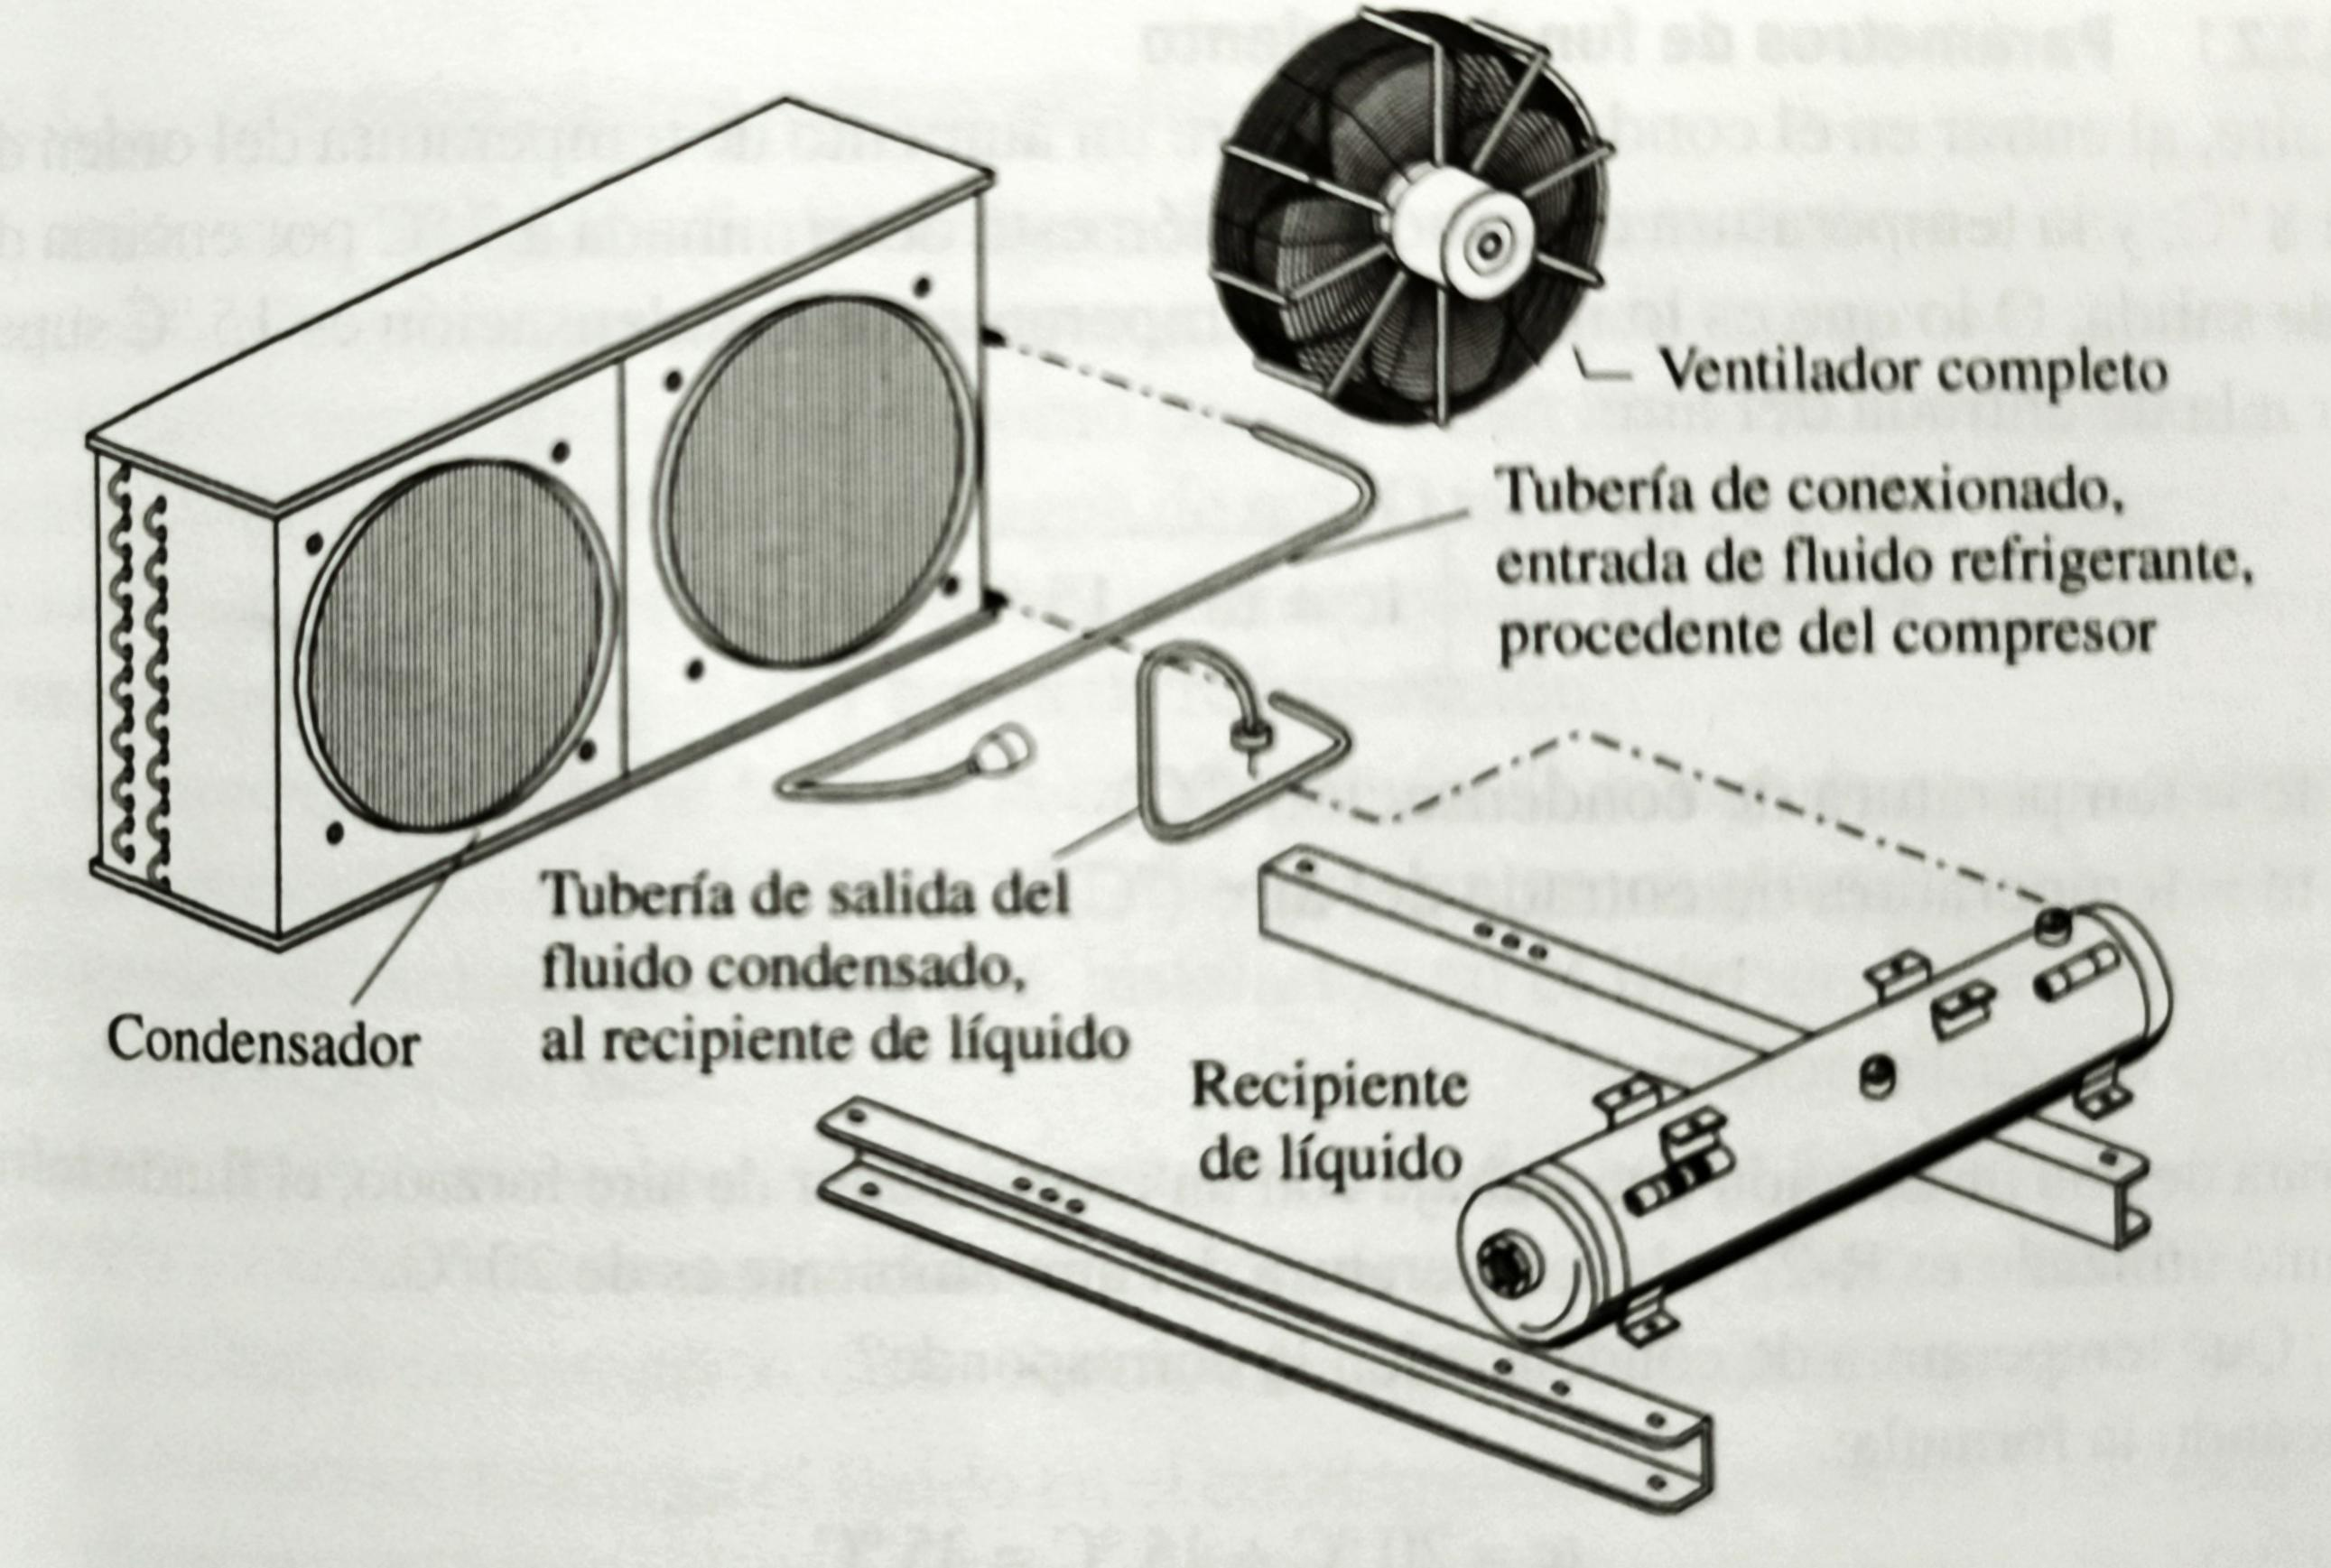
\includegraphics[width=.6\linewidth]{figuras/condensadores/condensador de aire forzado.jpg}
    \caption{Condensador de aire forzado}
    \label{fig:Condensador_de_aire_forzado}
\end{figure}

\subsubsection{Par\'ametros de funcionamiento}

El aire, al entrar al condensador, sufre un aumento de temperatura del orden de 7 u 8 \textcelsius, la temperatura de condensaci\'on est\'a determinada a 7 \textcelsius\ por encima de la de salida. O lo que es lo mismo, la temperatura de condensaci\'on es de 15 \textcelsius\ superior a la de entrada del aire.
\begin{equation*}
    tc = te + 15 \text{\textcelsius}
\end{equation*}
$tc = \text{temperatura de condensaci\'on (\textcelsius)}$\\
$te = \text{temperatura del aire (\textcelsius)}$\\
Estos par\'ametros tambi\'en podr\'iamos utilizarlos para determinar incondensables o suciedad, como en los condensadores por agua.

Por lo general, los condensadores por aire trabajan a temperaturas mayores que los que utilizan agua. Cuando hay variaciones importantes de la temperatura del aire, estos condensadores suelen llevar dispositivos de regulaci\'on (presostatos o termostatos), que act\'uan variando la velocidad de los ventiladores o parando uno o varios, seg\'un las necesidades.\\
\subsubsection{Mantenimiento}\\
A efectos de un buen mantenimiento, hay que evitar que se deposite suciedad entre las aletas, pues disminuir\'ia la transmisi\'on y por lo tanto el rendimiento. Se debe evitar que entre aletas se toquen porque esto dificultar\'ia el paso del aire, disminuyendo el rendimiento tambi\'en.

\subsection{Evaporativos}
Su funcionamiento se basa en la combinaci\'on de aire y de agua, a contracorriente, para efectuar la condensaci\'on. Se instalan en el exterior de la planta de refrigeraci\'on, aunque si hubiera que instalarlos en el interior, habr\'ia que prever las conducciones del aire.

\emph{Su rendimiento es funci\'on de la temperatura de bulbo h\'umedo del aire a la entrada y cuanto menor sea dicha temperatura mayor ser\'a el rendimiento}

Su funcionamiento es el siguiente:
\begin{enumerate}[1.]
    \item El compresor descarga el fluido en el condensador evaporativo y circula a trav\'es de un serpent\'in, el cual est\'a en el interior de una envolvente, que suele ser de material galvanizado.
    \item El ventilador (o ventiladores) hace circular el aire atmosf\'erico en sentido ascendente que aspira a trav\'es de las rejillas y lo descargan de nuevo, a la atm\'osfera, con lo cual pasa a trav\'es del serpent\'in enfri\'andolo.
    \item Asimismo, en la parte superior va instalada una l\'inea de agua con toberas, que la pulverizan sobre el serpent\'in. El agua cae al fondo del condensador y es aspirada por una bomba (1), que env\'ia nuevamente a las toberas.
\end{enumerate}
\begin{figure}[H]
    \centering
    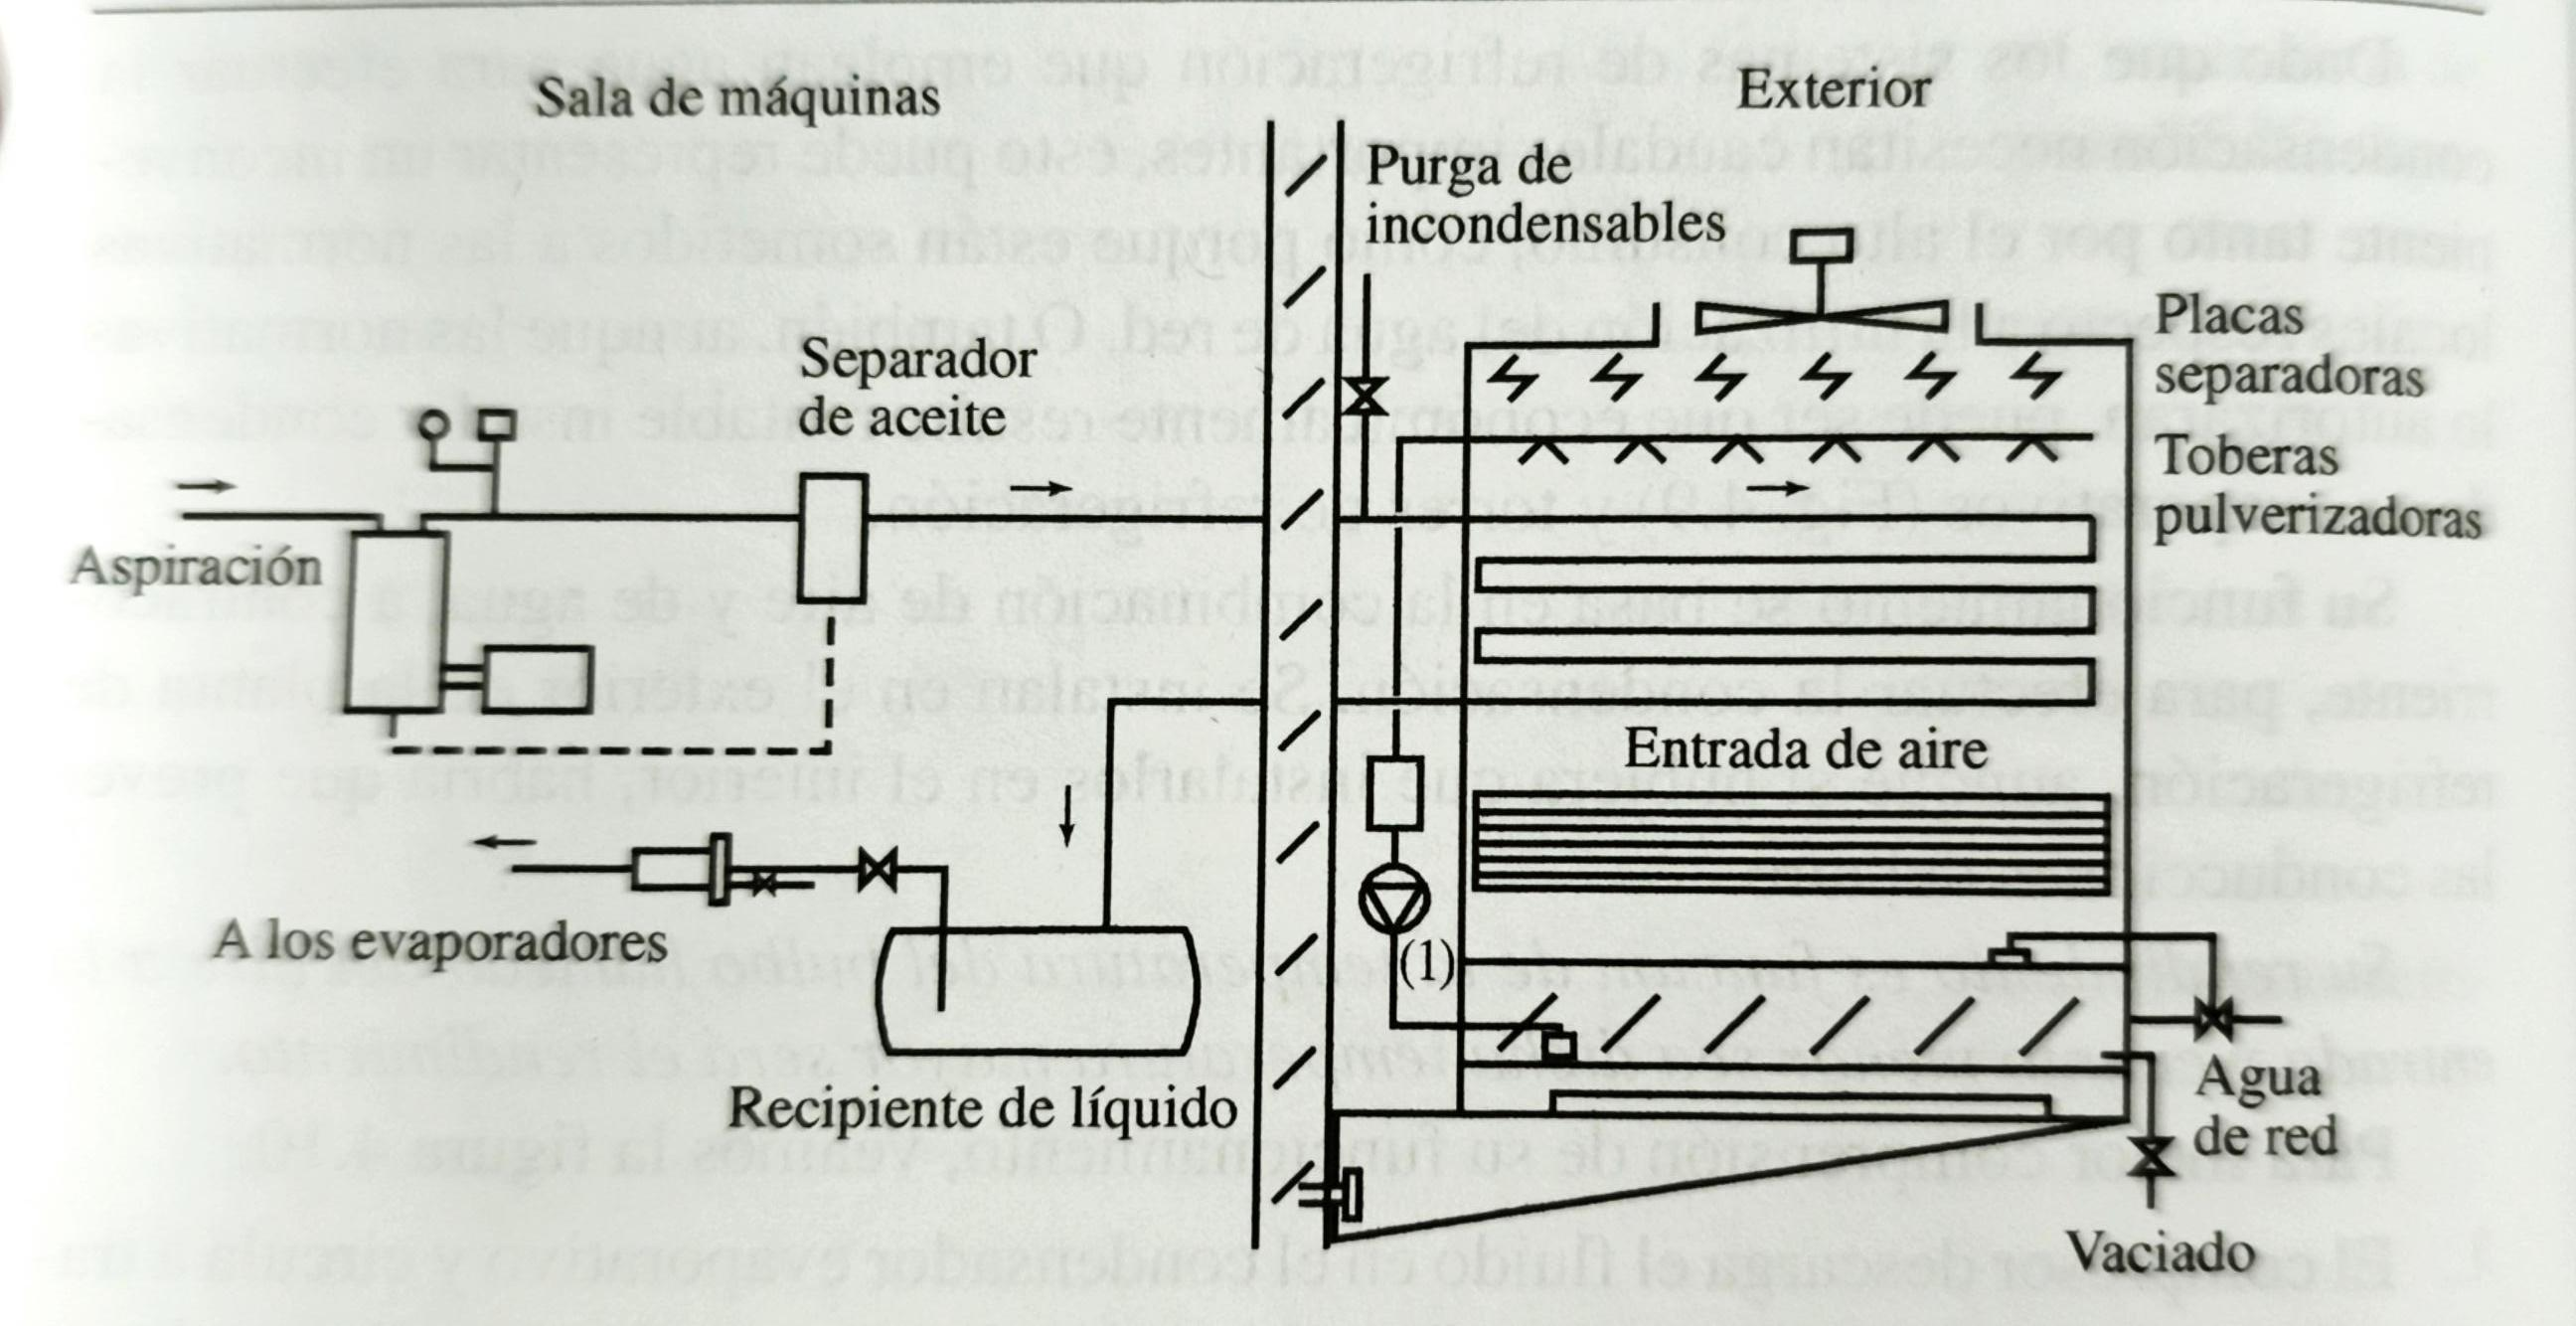
\includegraphics[width=0.7\linewidth]{figuras/condensadores/condensador evaporativo.jpg}
    \caption{Instalaci\'on de condensador evaporativo}
    \label{fig:Instalaci\'on de condensador evaporativo}
\end{figure}

Una parte del agua se pierde por evaporaci\'on a la atm\'osfera. Para evitar que sea importane esa p\'erdida, se colocan placas separadoras, que impiden que el agua por la acci\'on de los ventiladores sea descargada a la atm\'osfera, pues choca contra las placas y cae a la bandeja. De todos modos se pierde agua en el proceso, por lo que es necesario reponer el agua. Para ello, se coloca una v\'alvula en la l\'inea de alimentaci\'on (agua de red) controlada por un regulador de nivel (flotador).\\Tambi\'en hay que tener en cuenta que si la temperatura exterior donde se instale es muy baja, hay que a\~{n}adir soluci\'on de glicol o similar para disminuir su punto de congelaci\'on.\\Uno de los factores de los que depende el buen rendimiento de estos condensadores es mantener la superficie exterior del serpent\'in libre de dep\'ositos e incrustaciones.\\Como mantenimiento general, se deben realizar la limpieza de los pulverizadores y del serpent\'in. Tambi\'en se debe realizar purgas para disminuir la concentraci\'on de s\'olidos disueltos, en caso de no usar productos antiincrustantes.

\subsubsection{Selecci\'on de un condensador evaporativo}

Para seleccionar un condensador evaporativo debemos recurrir a las tablas y gr\'aficos de los fabricantes. Por ejemplo, para una instalaci\'on cuyos datos conocidos son los siguientes:
\begin{itemize}
    \item Capacidad a disipar = 180000 kcal/h
    \item Temperatura de condensaci\'on = 36\textcelsius
    \item Temperatura de bulbo h\'umedo = 20\textcelsius
    \item Fluido refrigerante = R-717 (amon\'iaco)
\end{itemize}
El proceso es el siguiente:
\begin{enumerate}[1.]
    \item Con el gr\'afico de la \autoref{fig:Factor k de correcci\'on} determinamos el factor ``K'' de correcci\'on, que est\'a relacionado con la temperatura de condensaci\'on y la temperatura de bulbo h\'umedo:
    \begin{figure}[H]
        \centering
        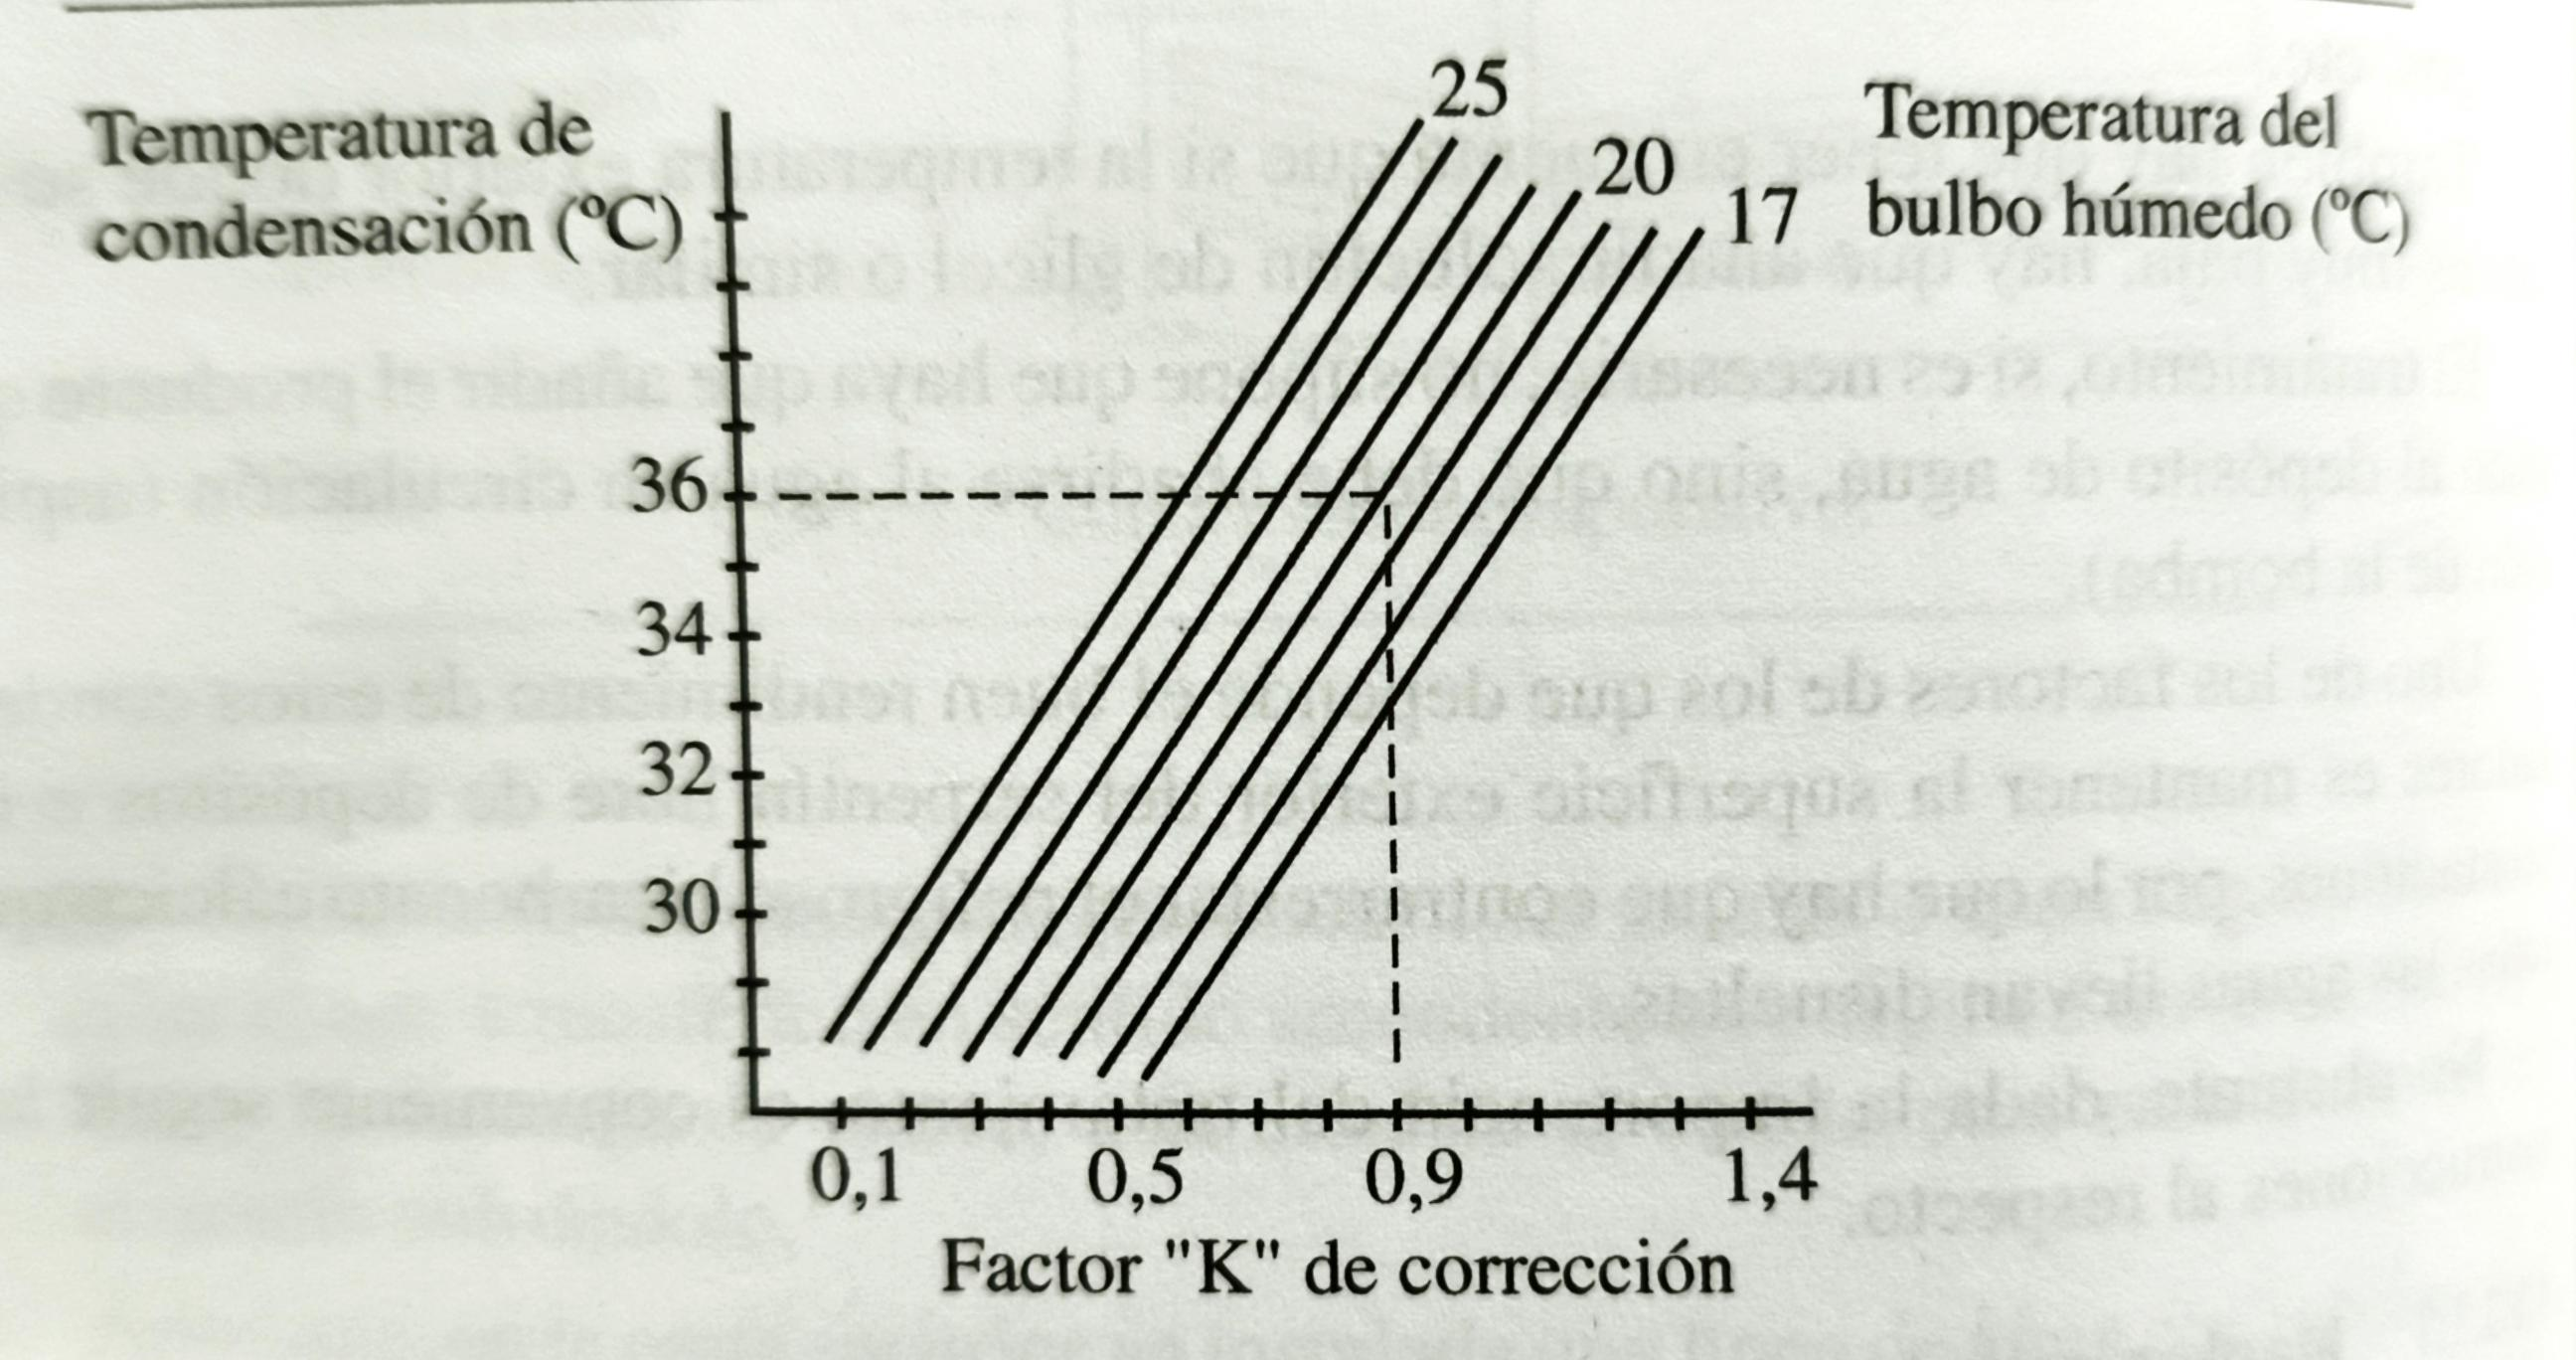
\includegraphics[width=0.6\linewidth]{figuras/condensadores/factor k de correcion.jpg}
        \caption{Factor ``K'' de correci\'on}
        \label{fig:Factor k de correcci\'on}
    \end{figure}
    \item Una vez obtenido el factor ``K'' = 0,9, hallamos la capacidad corregida:
    \begin{equation*}
        \frac{180000\ kcal/h}{0,9} = 200000\ kcal/h
    \end{equation*}
    \item A continuaci\'on, se debe seleccionar de cat\'alogo un modelo de condensador evaporativo que tenga una capacidad igual o mayor a la hallada.
\end{enumerate}
\subsection{Torres de refrigeraci\'on}
Se emplean en las instalciones de refrigeraci\'on y de acondicionamiento de aire. Se montan en el exterior del local.\\ Al igual que los condensadores evaporativos estos dispositivos utilizan aire y agua en su proceso. Pero a diferencia de los evaporativos estos elementos no realizan la condensaci\'on del fluido refrigerante de manera directa, sino que su misi\'on es enfriar el agua empleada para la condensaci\'on.
\begin{figure}[H]
    \centering
    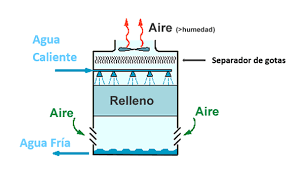
\includegraphics[width=.6\linewidth]{figuras/condensadores/torre de enfriamiento.png}
    \caption{Torre de enfriamiento}
    \label{fig:Torre de enfriamiento}
\end{figure}
\begin{wrapfigure}{r}{0.4\linewidth}
    \centering
    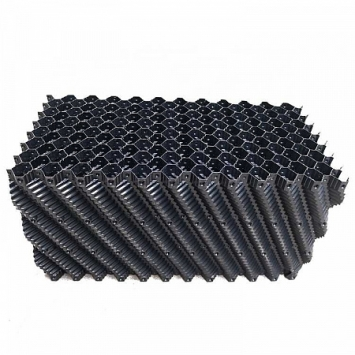
\includegraphics[width=0.6\linewidth]{figuras/condensadores/relleno.jpg}
    \caption{Panel o relleno}
    \label{fig:Panel o relleno}
\end{wrapfigure}
Tal como se ve en la \autoref{fig:Torre de enfriamiento} el agua a la salida del condensador es enviada mediante una bomba a la parte superior de la torre, donde es pulverizada por las toberas y cae sobre el panel o relleno (\autoref{fig:Panel o relleno}). Este relleno es un conjunto de l\'aminas soldadas entre s\'i y su funci\'on es aumentar la turbulencia de los flujos de aire y agua. El aire atmosf\'erico es impulsado por el ventilador (o ventiladores) en sentido ascendente y descargado a la atm\'osfera.\\
El agua se enfr\'ia porque cede su calor al aire; por ello, \textbf{cuanto m\'as baja sea la temperatura de bulbo h\'umedo, m\'as efectiva ser\'a la torre}, es decir m\'as humedad arrastr\'a el aire. El agua cae en la bandeja situada en la parte inferior y es aspirada por la bomba, que la env\'ia nuevamente al condensador. En la parte superior est\'an las placas separadores, cuya funci\'on es retener la mayor cantidad de agua del aire para su recuperaci\'on.

El control de la temperatura del agua del condensador se hace mediante la instalci\'on de una v\'alvula termost\'atica, la cual, seg\'un la temperatura que detecte, manda el agua a la torre o la recircula nuevamente al condensador. Otro sistema consiste en variar la velocidad de los ventiladores de la torre(con lo cual se var\'ia el caudal de aire) o bien actuando sobre el n\'umero de ventiladores que deben funcionar.

\section{Efectos del subenfriamiento}

El subenfriamiento moderado aumenta el efecto frigor\'ifico de nuestra instalaci\'on y, a su vez, asegura que el refrigerante llegue a la v\'avula de expansi\'on totalmente l\'iquido evitando el flash gas. El flash gas reduce la eficiencia del sistema y puede da\~{n}ar la v\'alvula de expansi\'on.El subenfriamiento tambi\'en nos puede dar idea de como esta funcionando el condensador o que problemas podr\'ia tener, seg\'un aumente o disminuya.

Un \emph{subenfriamiento bajo} puede ser causa de:
\begin{itemize}
    \item Fuga de refrigerante
    \item Lineas de l\'iquido demasiado largas (mucha ca\'ida de presi\'on)
    \item Flujo de aire en el condensador bajo
    \item Altas temperaturas de ambientales alrededor de las l\'ineas de l\'iquido
\end{itemize}
Un \emph{subenfriamiento alto} puede ser por:
\begin{itemize}
    \item Sobre carga de refrigerante
    \item Obstrucci\'on en la l\'inea de l\'iquido
    \item Temperaturas exteriores bajas
\end{itemize}
Un subenfriamiento alto podr\'ia causar que el condensador se inunde, disminuyendo el intercambio de calor latente y elevando la presi\'on en el mismo. Esto har\'ia que la presi\'on de descarga del compresor aumente y por lo tanto su trabajo.\\El aumento en la producci\'on frigor\'ifica gracias al subenfriamiento estar\'a determinado por el efecto refrigerante del fluido por cada kilogramo. Este aumento no ser\'a el mismo para una instalaci\'on con R22 y otra con R717, en la cual ambas tiene el mismo subenfriamiento.

\section{Selección del condensador}

Se trata de determinar la capacidad nominal del condensador que se debe instalar. Para ello se deben utilizar tablas de fabricantes, que las elaboran seg\'un datos que obtienen en las pruebas que realizan.

\subsubsection{Ejemplo de aplicaci\'on:}

Datos de la instalaci\'on:
\begin{itemize}
    \item Capacidad del evaporador: 28000 kcal/h
    \item Temperatura de evaporaci\'on: -10\textcelsius
    \item Temperatura de condensaci\'on: 35\textcelsius
    \item Temperatura del aire ambiente: 20\textcelsius
    \item Fluido refrigerante: R22
\end{itemize}
Para determinar la capacidad nominal del condensador hacemos uso de la siguiente ecuaci\'on:
\begin{equation}
    Qn = Qe \cdot Fc \cdot Fr \cdot Fa \cdot \frac{15}{Dt}
\end{equation}

$Qn = \textit{capacidad nominal del condensador}$\\
$Qe = \textit{capacidad del evaporador}$\\
$Fc = \textit{factor de calor de compresi\'on}$\\
$Fr = \textit{factor de refrigerante}$\\
$Fa = \textit{factor de altitud}$\\
$Dt = \textit{diferencia de temperaturas (tc - ta)}$\\
\begin{enumerate}[a.]
    \item El factor de calor de compresi\'on (Fc), se obtiene de la gr\'afica siguiente:
    \begin{figure}[H]
        \centering
        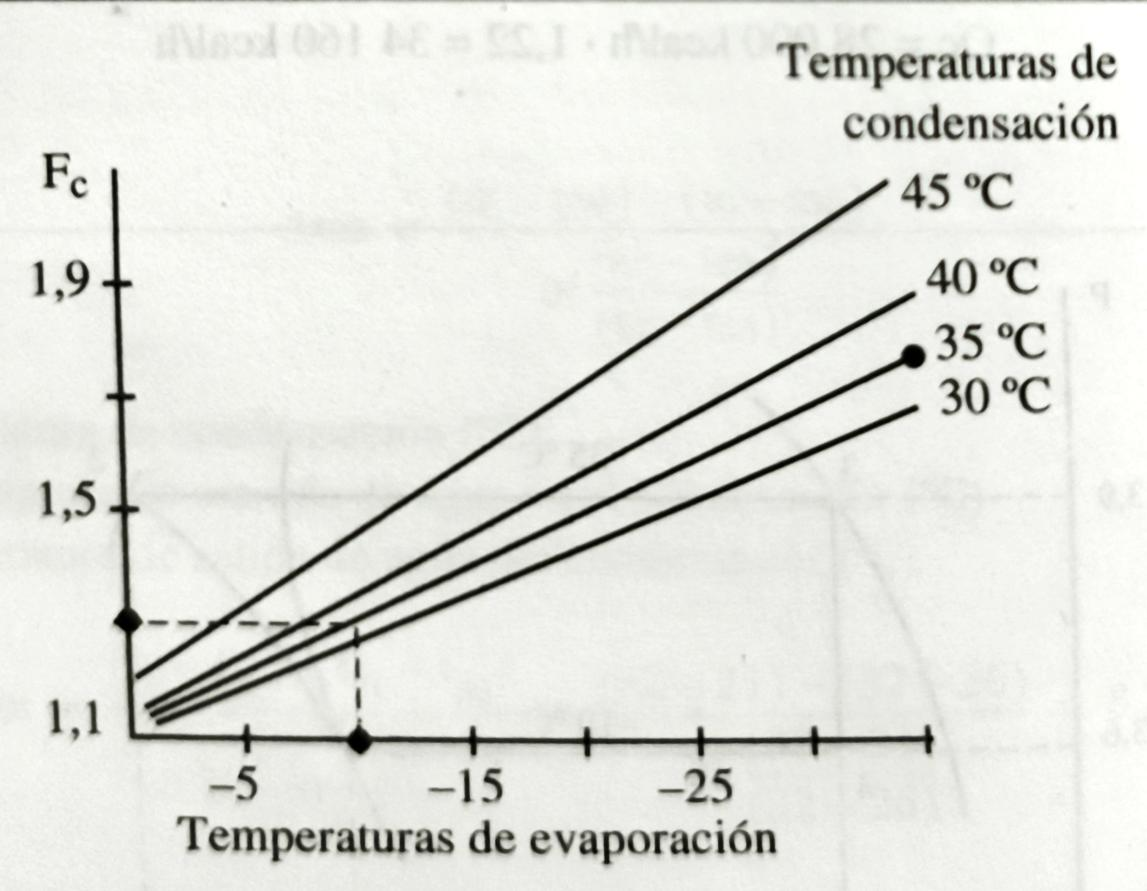
\includegraphics[width=.6\linewidth]{figuras/condensadores/factor de calor de compresion.jpg}
        \caption{Factor de calor de compresi\'on}
        \label{fig:Factor de calor de compresi\'on}
    \end{figure}
    Con lo que $Fc = 1,3$
    \item Factor del refrigerante (Fr), seg\'un la tabla del fabricante:
    \begin{figure}[H]
        \centering
        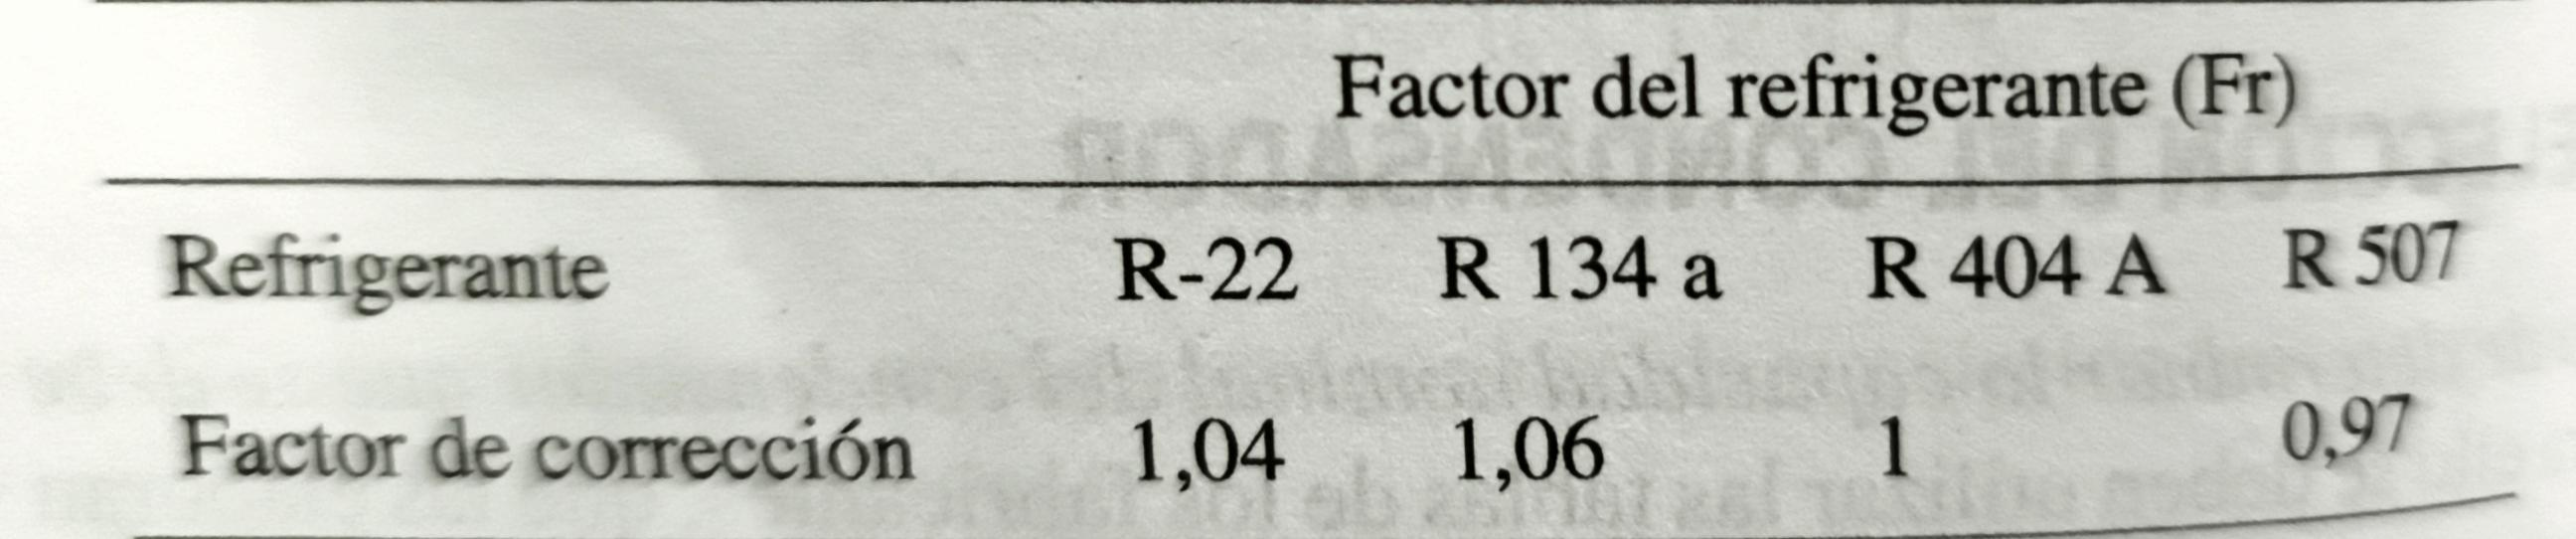
\includegraphics[width=.7\linewidth]{figuras/condensadores/factor del refrigerante.jpg}
        \caption{Factor del refrigerante}
        \label{fig:Factor del refrigerante}
    \end{figure}
    Con lo cual $Fr = 1,04$
    \item Para obtener el factor de altitud (Fa), recurrimos a la siguiente tabla:
    \begin{figure}[H]
        \centering
        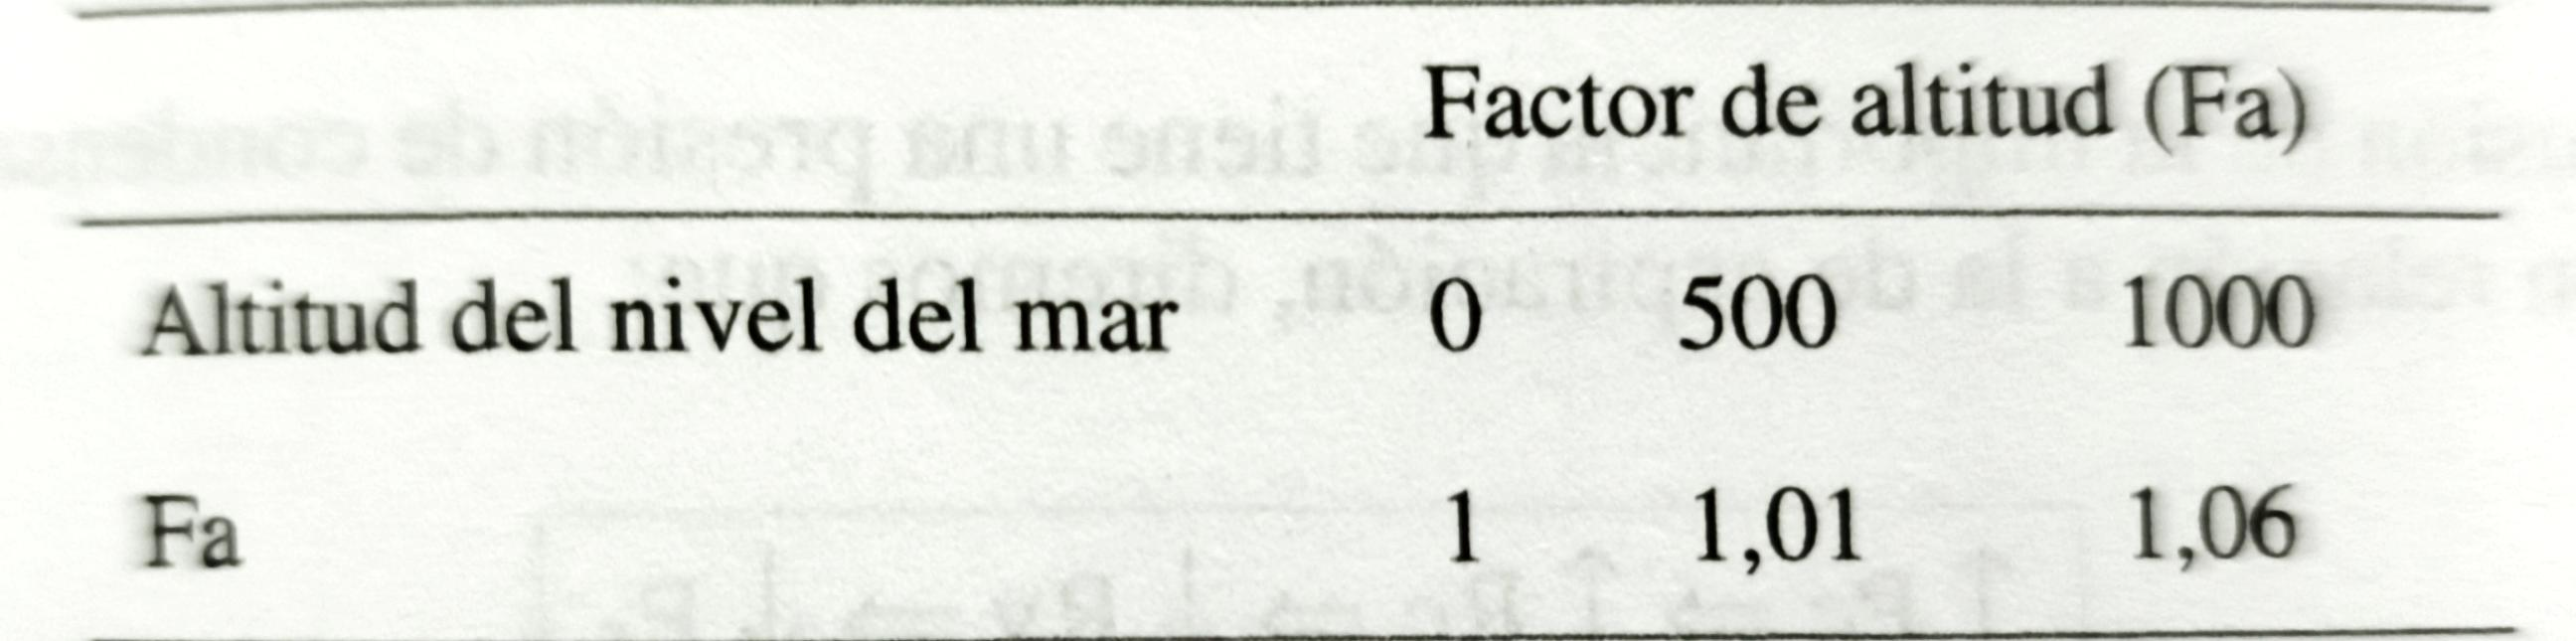
\includegraphics[width=.6\linewidth]{figuras/condensadores/factor de altitud.jpg}
        \caption{Factor de altitud}
        \label{fig:Factor de altitud}
    \end{figure}
    Con lo cual $Fa = 1$
    \item $Dt$ es la diferencia entre la temperatura de condensaci\'on y la de entrada del aire; en este caso:
    \begin{equation*}
        Dt = 35 - 20 = 15 \text{\textcelsius}
    \end{equation*}
    Con lo que $\tfrac{15}{Dt} = \tfrac{15}{15} = 1$
    \item Con los valores obtenidos en las correspondientes tablas, aplicando la \ref{eq:calor} obtenemos que:
    \begin{equation*}
        Qn = 28000\ kcal/h \cdot 1,3 \cdot 1,04 \cdot 1 \cdot 1 = 37856\ kcal/h
    \end{equation*}
\end{enumerate}